% arara: xelatex: { shell: yes }
% arara: biber
% arara: makeglossaries
% arara: xelatex: { shell: yes }
% arara: xelatex: { synctex: true, shell: yes }
%=========================================================================
%------------------THESIS TEMPLATE OF Dr. DENISOV Sergey------------------
%=========================================================================
%------------------------UNIVERSITÉ DE BORDEAUX---------------------------
%------------------------------Talence------------------------------------
%---------------------------- 2013-2015-----------------------------------
%-------------------------BASED ON BOOK.CLS-------------------------------
%------------------XELATEX or LULATEX+BIBER+MAKEGLOASSARIES-------------------------
%=========================================================================
\documentclass[a4paper,12pt,onecolumn,notitlepage,openright,twoside,singlespacing]{thesis-Bordeaux}

%SHORTENINGS
%-------------------------------------------------------
\DeclareMathOperator{\erf}{erf}
\DeclareMathOperator{\exc}{exc}
\DeclareMathOperator{\decay}{decay}
\newcommand{\eg}{e.\,g.\xspace}
\newcommand{\ie}{i.\,e.\xspace}
\newcommand{\per}{\,\%\xspace}
\newcommand{\temp}{$^\circC\xspace$}
\newcommand{\chlD}{$\rm CDCl_3$\xspace}
\newcommand{\chl}{$\rm CHCl_3$\xspace}
\newcommand{\dcm}{$\rm CH_2Cl_2$\xspace}
\newcommand{\acetonitrile}{$\rm CH_3CN$\xspace}
%=======================================================
\usepackage{csquotes}
\usepackage[backend=biber,bibencoding=utf8, indexing=cite, style=custom-numeric-comp, sorting=none,maxbibnames=99]{biblatex}
%backref=false,
%backrefstyle=three
\addbibresource{bibliography/thesis-bib.bib}


\DefineBibliographyStrings{english}{%
    backrefpage  = {see \lowercase{p}.}, % for single page number
    backrefpages = {see \lowercase{p}p.} % for multiple page numbers
}

\DeclareNameAlias{sortname}{last-first}
\DeclareNameAlias{default}{last-first}

%\AtBeginBibliography{\renewcommand*{\mkbibnamelast}[1]{\MakeUppercase{#1}}}

%\DeclareFieldFormat{volume}{\def\tmp##1##2{\ifinteger{##1}{\bibstring{volume}\addspace##1##2}{##1##2}}\expandafter\tmp#1}
%\DefineBibliographyStrings{english}{%
%	number = {\lowercase{v}ol\adddot}, % avoid capitalization after dots.
%	issue  = {\lowercase{i}ss\adddot}, % avoid capitalization after dots.
%}

\DeclareFieldFormat
[article]
{journaltitle}{\textit{#1}}
\DeclareFieldFormat
[article]
{volume}{#1}


\usepackage{imakeidx}
\makeindex[intoc,name=pms,title=General,columns=2]
\makeindex[intoc,name=cite,title=Author Index,columns=2]
\indexsetup{level=\chapter*,toclevel=chapter,noclearpage}

%Include authors from bibliography to author index.
\DeclareIndexNameFormat{default}{%
	\nameparts{#1}%
	\usebibmacro{index:name}
	{\index[cite]}
	{\namepartfamily}
	{\namepartgiven}
	{\namepartprefix}
	{\namepartsuffix}}

%\DeclareIndexNameFormat{nondefault}{%
%\usebibmacro{index:name}{\nocite[cite]}{#1}{#3}{#5}{#7}}  

%Glossaries
\usepackage[nonumberlist,acronym,toc,nomain,nopostdot,nogroupskip]{glossaries}
\input{Settings/abbr}
\makeglossaries
%\usepackage[english,french,italian,russian,swedish,german]{babel}
\usepackage[english,french]{babel}

%Language support and main font
\addto\captionsfrench{\def\tablename{Tableau}}



\usepackage{amsmath}
%For LuaLaTeX
%\usepackage{fontspec}
%\setmainfont{Times New Roman} 
%\setmathrm{Times New Roman}
%\setmathsf{Times New Roman}
%\setmathtt{Times New Roman}
%\setboldmathrm{Times New Roman}



%For XeLaTeX
\usepackage{mathspec}
\setmainfont[Mapping=tex-text, Numbers={Lining,Proportional}]{Times New Roman} 
\setmathsfont(Digits)[Numbers={Lining,Proportional}]{Times New Roman}
\setmathsfont(Latin)[Scale=MatchLowercase]{Times New Roman}
\setmathsfont(Greek)[Scale=MatchLowercase]{Times New Roman}
\setmathrm{Times New Roman}



\usepackage{ifthen}
\usepackage{lipsum}
\usepackage{color,soul}
\usepackage{pdfpages}
\usepackage{pdflscape}

\makeatletter
\renewcommand*\l@subsection{\@dottedtocline{2}{3.8em}{4.3em}}% Used to be {3.8em}{3.2em}
\renewcommand*\l@table{\@dottedtocline{1}{1.5em}{2.8em}}
\renewcommand*\l@figure{\@dottedtocline{1}{1.5em}{2.8em}}
\makeatother


%This packages are used just for showing some examples of code in this manual, but not used for thesis itself. So they can be deleted from the thesis
\usepackage{xcolor}
\usepackage{listings}
\lstset{backgroundcolor=\color{green!3},language=[LaTeX]Tex,commentstyle=\color{green!30!black!80},basicstyle=\footnotesize,breaklines=true,numbers=left, numberstyle=\tiny, stepnumber=1, numbersep=10pt}
%-----------------------------------------------------------------------------------

\begin{document}
\frontmatter

\pagestyle{plain}
\selectlanguage{english}

%Title page
%Set data of title page
\setthesisSpeciality{LASERS, MATIÈRE ET NANOSCIENCES}

\setThesisschool{\'{E}COLE DOCTORALE DES SCIENCES PHYSIQUES ET DE L'ING\'{E}NIEUR (SP1)}

\setAuthorname{Nom Prénom}

\setThesistitle{Thesis name enter here in french}

\setThesistitleO{Thesis name enter here in english}

%\setCodirector{No}

\setDirector{Dr. Director. First}
%If there is no second director Type 'No' instead of 'Dr. Director. Second'
\setCodirector{Dr. Director. Second}

\setThesisdate{1 avril 2015}

\setCommittee{
	\begin{tabular}{lll}
		\hspace{-2.3mm}M.  ONE, One& Université de  Bordeaux&  Président\\
		\hspace{-2.3mm}Mme. TWO, Two&  Université de  Bordeaux& Rapporteur\\
		\hspace{-2.3mm}M. THREE, Three&  Université de  Bordeaux& Rapporteur\\
		\hspace{-2.3mm}M. FOUR, Four&  Université de  Bordeaux & Examinateur\\
		\hspace{-2.3mm}M. FIVE, Five&  Université de  Bordeaux & Directeur\\
		\hspace{-2.3mm}M. SIX, Six&  Université de  Bordeaux & Co-directeur\\
	\end{tabular}}


\setResume{French résume}

\setCles{Mots-clés}

\setAbstract{English abstract}

\setKeys{Keywords}

\setLabadress{Laboratoire Ondes et Matière d'Aquitaine Université de Bordeaux, UMR CNRS 5798 351 cours de la Liberation, 33405 Talence, France}

%Generate title page
\titlePage
\newpage

%Dedication
\addcontentsline{toc}{chapter}{Dedication}
\begin{middleOfPage}
Dedicated to mankind...:)
\end{middleOfPage}
\newpage

%Epigraph
\chapter*{Preface}
\addcontentsline{toc}{chapter}{Preface}
\selectlanguage{french}


\epigraph{Ce que nous connaissons est \textbf{peu de chose}, ce que nous ignorons est\textbf{ immense}.}{French mathematician and astronomer, Pierre-Simon de Laplace (1749--1827)\index[cite]{Laplace, P.-S.}}



\epigraph{Il piacere della vita è imparare.}{ Italian scholar and poet, Francesco Petrarca (1304--1374) \index[cite]{Petrarca, F.}}


\vspace{10mm}
\selectlanguage{english}
\lipsum[1-5]
\newpage

%Acknowledgements
\chapter*{Acknowledgments}
\addcontentsline{toc}{chapter}{Acknowledgments}
\selectlanguage{english}

\lipsum[1-5]
\newpage

%Extended resume
\renewcommand*\thesection{\arabic{section}}
% !TeX spellcheck = fr_FR

% Extened abstract in french for english written manuscripts.s
\chapter*{Résumé en français}
\selectlanguage{french}
\frenchspacing
\renewcommand\thefigure{\Roman{figure}} 
\renewcommand\thetable{\Roman{table}}  

\addcontentsline{toc}{chapter}{Résumé}

% !TeX spellcheck = fr_FR
\section{Introduction}
\lipsum[1-3]


%etc.....

%\input{parts/front/resume/someother-section}

\renewcommand\thefigure{\thechapter.\arabic{figure}}
\renewcommand\thetable{\thechapter.\arabic{table}}

\nonfrenchspacing
\selectlanguage{english}

\renewcommand*\thesection{\arabic{chapter}.\arabic{section}}


% TableofContents
\tableofcontents
\listoffigures
\listoftables
\selectlanguage{english}
\mainmatter
\pagestyle{fancy}

%Chapter I
% !TeX spellcheck = en_GB
\chapter{How to use thesis template}
\label{ch:how-to-use}
%------------------------------------------------------
\epigraph{L'art c'est \textbf{moi} -- la science c'est \textbf{nous}.}{french physiologist, Claude Bernard (1813--1878) \index[cite]{Bernard, C.}}
%======================================================
\startcontents[chapter]
\printcontents[chapter]{}{-1}{\setcounter{tocdepth}{3}}
\newpage


\section{General Description}
This thesis template was done in 2013-2015 according to the rules of Université de Bordeaux. It can be compiled with two different chains:
\begin{enumerate}
	\item xelatex -- beamer -- makeglossaries -- xelatex -- xelatex
	\item lualatex -- beamer -- makeglossaries -- lualatex -- lualatex
\end{enumerate}

I as author recommend to use \textbf{MiKTeX} or \textbf{TeX Live} as a \LaTeX distributions, and from my opinion best editors for general purposes are TeXStudio or TeXMaker.


\subsection{Organization}

Thesis is divided in several part:
\begin{enumerate}
	\item Settings
	\item Front Matter (Title Page, Dedication, etc., contents, list of tables and figures)
	\item Main Matter ( Chapters, Appendixes)
	\item Back Matter (Bibliography, Acronyms)
\end{enumerate}

The thesis is divided in to chapters, but not in parts.

The settings of thesis is mainly kept inside of thesis class \textit{thesis-bordeax.cls}. Settings for bibliography could be found in \textit{settings/Bib.tex}, for fonts \textit{settings/Fonts.tex}.

\subsection{ARARA}
I highly recommend to use \textbf{Arara\footnote{Automation of \LaTeX compilation}}. To add Arara command to TEXMaker this nice \textit{post} could be used: \href{http://tex.stackexchange.com/a/107995/43831}{http://tex.stackexchange.com/a/107995/43831}


\section{Floats}

\subsection{Figures/Images/Drawings}
I recommend to use \textit{TikZ}+\textit{pgfplots} packages to built graphs. All presented graphs in this manual are made using this two packages (see \textit{figures} folder for corresponding \textit{tex} file).\par

There are several ways to insert figures in thesis:

\begin{itemize}
	\item Standard way
	\begin{lstlisting}
	\begin{figure}
	\centering
	%\includegraphics[width=6cm]{Name-of-file}
	\caption{Caption.}
	\label{fig:firstFig}
	\end{figure}
	\end{lstlisting}
	
	\item Using \lstinline|\inputfigure| command:
	
	\lstinline|\inputfigure[scale 0 to 1]{File Name}[Caption][Label][type of file pdf, png]|, example: \lstinline|\FloatBarrier\inputfigure[.5]{Chapter1/streak-cameraTIKZ}[Principle scheme of a conventional streak camera][streak-camera][pdf] \FloatBarrier|
	
	\FloatBarrier
	\inputfigure[.5]{Chapter1/streak-cameraTIKZ}[Principle scheme of a conventional streak camera][streak-camera][pdf]
	\FloatBarrier
	
	
	To get an idea hot \textit{TikZ} package works see \textit{figures/Chapter1/streak-cameraTIKZ.tex}:
	
	
	
	\item Using \lstinline|\inputfiguresH}[scale]{Name1}{Name2}[Caption1][Caprtion2][Label1][Label2][Height1][Height1]| command:
	
	
	
	\begin{lstlisting}
	\FloatBarrier
	\inputfiguresH[1]{Chapter1/RuII-GS-bleaching.pdf}{Chapter1/RuII-anth-3growth.pdf}[\acrshort{TRABS} kinetics of ground state bleaching changes for \textbf{2} at $485$\,nm in \acetonitrile ($\lambda_{exc}=465$\,nm)][\acrshort{TRABS} kinetics of anthracene triplet grow-in for \textbf{2} at $430$\,nm in \acetonitrile ($\lambda_{exc}=465$\,nm)][RuII-GS-bleaching][RuII-anth-3growth][5][5]
	\FloatBarrier
	\end{lstlisting}
	
	
	\FloatBarrier
	\inputfiguresH[1]{Chapter1/RuII-GS-bleaching.pdf}{Chapter1/RuII-anth-3growth.pdf}[\acrshort{TRABS} kinetics of ground state bleaching changes for \textbf{2} at $485$\,nm in \acetonitrile ($\lambda_{exc}=465$\,nm)][\acrshort{TRABS} kinetics of anthracene triplet grow-in for \textbf{2} at $430$\,nm in \acetonitrile ($\lambda_{exc}=465$\,nm)][RuII-GS-bleaching][RuII-anth-3growth][5][5]
	\FloatBarrier
	
	
\end{itemize}


\subsection{Tables}


\begin{lstlisting}
\begin{table}[h!]
\addtocounter{totaltables}{1}
\caption{Characteristic time, distance and energy ranges for chemistry and physics.}
\label{table:Ranges}
\centering
\begin{tabular}{|x{2cm}|>{\centering\arraybackslash}x{2.5cm}|>{\centering\arraybackslash}x{3.7cm}|>{\centering\arraybackslash}x{3.1cm}|}

\hline  
&  Time range, s&  Size range, m&  Energy range, eV\\ 
\hline  
Chemistry&  $\rm 10^{-15} - ^*$& $\rm 10^{-10} -10^{1}$  (11~orders) & $\rm 10^{-4} -10^{0}$ (4~orders) \\

\hline  

Physics&  $\rm 10^{-44} -10^{18}$ ($\rm >50$~orders)& $\rm 10^{-35}-10^{-18} -10^{26}$ ($\rm >40$~orders) & up to $\rm 10^{70}$ \\

\hline 
\end{tabular} 
\end{table}
\end{lstlisting}

\begin{table}[h!]
\addtocounter{totaltables}{1}
\caption{Characteristic time, distance and energy ranges for chemistry and physics.}
\label{table:Ranges}
\centering

\begin{tabular}{|x{2cm}|>{\centering\arraybackslash}x{2.5cm}|>{\centering\arraybackslash}x{3.7cm}|>{\centering\arraybackslash}x{3.1cm}|}

\hline  
&  Time range, s&  Size range, m&  Energy range, eV\\ 
\hline  
Chemistry&  $\rm 10^{-15} - ^*$& $\rm 10^{-10} -10^{1}$  (11~orders) & $\rm 10^{-4} -10^{0}$ (4~orders) \\
 
\hline  

Physics&  $\rm 10^{-44} -10^{18}$ ($\rm >50$~orders)& $\rm 10^{-35}-10^{-18} -10^{26}$ ($\rm >40$~orders) & up to $\rm 10^{70}$ \\
 
\hline 
\end{tabular} 
\end{table}

\begin{table}[h!]
\caption{Photophysical properties of Ru(II) complexes in \acetonitrile.}
\label{tab:Ru-properties}

\begin{ThreePartTable}
\centering
%6 columns
\begin{tabu}{{|[2pt] c|c|c|c|c|c|[2pt]}}

\tabucline[2pt]{-}
complex & $\lambda_{em.\,max}$, nm\tnote{a} & $ \Phi_{air}$\tnote{b}&$\Phi_{degas}$\tnote{c} & $\tau$, $\mu$s\tnote{d} & $ K_{eq}$\tnote{f}\\
\tabucline[2pt]{-}

\textbf{1} &686&$2.2 \times 10^{-3}$&$1.3 \times 10^{-2}$& $2.7\pm0.3$&--\\

\tabucline[1pt]{-}

\textbf{2}& 686&$4 \times 10^{-4}$&$9.5 \times 1.3^{-2}$ & $\rm 75\times 10^{-6}$\tnote{e}; $42\pm2$&$15.2\pm2$\\

\tabucline[2pt]{-}


\end{tabu}
\begin{tablenotes}
\footnotesize
\item[a] Recorded on streak camera and uncorrected.

\item[b]  Luminescence QY in air-equilibrated $\rm CH_3CN$ solution \textit{cf.} $\rm [Ru(bpy)_3]^{2+}$ in $\rm H_2O$ (bpy = 2,2'--bipyridine).

\item[c]Luminescence QY in degassed $\rm CH_3CN$ solution \textit{cf.} $\rm [Ru(bpy)_3]^{2+}$ in $\rm H_2O$.

\item[d] MLCT luminescence lifetime in dilute degassed $\rm CH_3CN$.

\item[e] Determined \textit{via} transient absorption spectroscopy in degassed $\rm CH_3CN$. 

\item[f] Excited-state equilibrium constant. 
\end{tablenotes}


\end{ThreePartTable}

\end{table}


\section{Bibliography, Citations and Author Index}

The bibliography print commands are located in \textit{backmatter.tex} file:

\begin{lstlisting}
\addcontentsline{toc}{chapter}{\bibname}
\begingroup
\setstretch{1}
\setlength\bibitemsep{0pt}
\renewcommand*{\bibfont}{\small}
\sloppy %Line breaking
\printbibliography
\endgroup
\end{lstlisting}

The settings are located in \textit{settings/Bib.tex} file. The library itself is stored in \textit{bibliography.thesis-bib.bib} file:

\begin{lstlisting}
@phdthesis{Ducrot-thesis,
author = {Ducrot, A.},
school = {Universit\'{e} Bordeaux 1},
title = {{Synthèses et études de systèmes supramoléculaires photocommutables : récepteurs à ion et molécules entrelacées}},
year=2012,
}

@article{Haas-1971,
author = {Haas, Y. and Stein, G.},
journal = {J. Phys. Chem.},
number = {24},
title = {{Pathways of radiative and radiationless transitions in europium(III) solutions. Role of solvents and anions}},
volume = {75},
year = {1971}
}
\end{lstlisting}

To cite any item from the library the citation command should be used \lstinline|\cite{label}| for example \lstinline|\cite{Berlman1971}| which gives: \cite{Berlman1971}.

The authors from the article automatically added to \textit{author index} by this code located in \textit{settings/Bib.tex}:

\begin{lstlisting}
\usepackage{imakeidx}
\makeindex[intoc,name=cite,title=Author Index,columns=2]
\indexsetup{level=\chapter*,toclevel=chapter,noclearpage}

%Include authors from bibliography to author index.
\DeclareIndexNameFormat{default}{%
\usebibmacro{index:name}{\index[cite]}{#1}{#3}{#5}{#7}}

\DeclareIndexNameFormat{nondefault}{%
\usebibmacro{index:name}{\nocite[cite]}{#1}{#3}{#5}{#7}}  
\end{lstlisting}



\section{Abbreviations}
The acronyms are kept in the file \textit{Settings/abbr.tex}, which you can find  inside of \textit{Bib.tex} file:

\begin{lstlisting}
%Glossaries
\usepackage[nonumberlist,acronym,toc,nomain,nopostdot,nogroupskip]{glossaries}
\input{Settings/abbr}
\makeglossaries
\end{lstlisting}

To set up new acronym this code should be used \lstinline|\newacronym{CSS}{CSS}{Charge Separated State}|.

There are tree ways to use acronym in the text:
\begin{enumerate}
	\item short \lstinline|\acrshort{CSS}| -- \acrshort{CSS}
	\item long  \lstinline|\acrlong{CSS}| -- \acrlong{CSS}
	\item full \lstinline|\acrfull{CSS}| -- \acrfull{CSS}
\end{enumerate}
  
At the of thesis the full list of acronyms will be printed:
\begin{lstlisting}
%Glossary
\glsaddall
\renewcommand*{\glsgroupskip}{}
\printglossary[title=Abbreviations, toctitle=Abbreviations, type=\acronymtype, style=list]
\end{lstlisting}

\section{Indexes}

In the thesis two indexes are created in \textit{settings/Bib.tex} file:

\begin{lstlisting}
\usepackage{imakeidx}
\makeindex[intoc,name=pms,title=General,columns=2]
\makeindex[intoc,name=cite,title=Author Index,columns=2]
\indexsetup{level=\chapter*,toclevel=chapter,noclearpage}
\end{lstlisting}

The \textit{cite} index is used to store cited authors, \lstinline|\cite{}| command automatically adds author in author index. To add manually this command should be used \lstinline|\index[cite]{Bernard, C.}|


The indexes are printed in the of thesis:

\begin{lstlisting}
%INDEXES
\printindex[cite]
%\printindex[pms]
\end{lstlisting}


\section{References}

The package \textit{hyperref} is used to create references in the thesis. To create a reference this commands are used:
\begin{itemize}
	\item reference to chapter, section, etc. \lstinline|\ref{label}|, for example reference to chapter \textit{How to use thesis template}  \lstinline|\ref{ch:how-to-use}| will give \ref{ch:how-to-use}, or figure....
	\item reference to chapter, section, figure, table etc. page \lstinline|p.~\page ref{ch:how-to-use}| -- p.~\pageref{ch:how-to-use}. 
\end{itemize}


\stopcontents[chapter]

%Chapter II
% !TeX spellcheck = en_GB
\chapter{Chapter Example}
\label{ch:2chapter}
%------------------------------------------------------
\epigraph{Some very clever idea }{Very clever man \index[cite]{Clever Man}}
%======================================================
\startcontents[chapter]
\printcontents[chapter]{}{-1}{\setcounter{tocdepth}{3}}
\newpage

In this chapter (Chapter~\ref{ch:2chapter}) will be presented unrelated data...I'm really sorry for that.

\section{Molecules}
\label{sec:2ch-molecules}

Please find structures of molecules\footnote{Made in LaTeX as well.} which were used in the study (see Fig.~\ref{fig:molecules}). The data is presented in section \ref{sec:2ch-data} on p.~\pageref{sec:2ch-data}. 
\inputfigure[.5]{Chapter2/molecules}[Studied molecules][molecules][pdf]


\section{Data}
\lettrine[lraise=0.1]{W}{e} discussed earlier that systems studied in this work are photo-activated (\acrshort{RET}, \acrshort{REET}, \acrshort{PET}, Photoisomerization). It simply means that system should be excited from its ground state to some electronic excited state, because only upon being in the excited state the system could be active from the point of displaying useful property. At room temperature thermal energy is not adequate to significantly populate electronically excited states.\par

Here we would like to spent some time to discuss such terms as \emph{state} and the~term~\emph{excited~state}.\par

\begin{wrapfigure}{l}{0.5\linewidth}
	\centering
	\centering
	\addtocounter{totalfigures}{1} 
	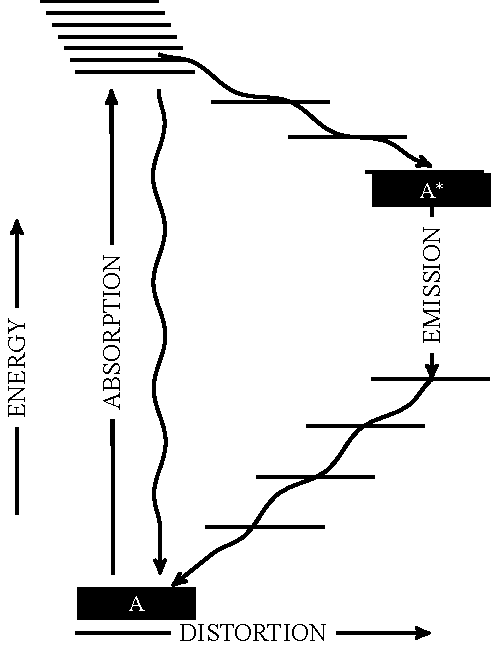
\includegraphics[width=.6\linewidth]{figures/Chapter2/energydistoration}
	\caption{Energy versus distortion diagram\,\cite{adamson-1983}.}
	\label{fig:energydistoration}	
\end{wrapfigure}

The work of Adamson\cite{adamson-1983} we will helpful in the discussion.\par

The word \emph{state} has two different usages in science. To the spectroscopist, the state of a molecule is defined by quantum numbers. He will use term designations and thus speak of the $^2P_{1/2}$ state of the sodium atom or the $^3\Sigma^-_g $ state of $\rm O_2$. In the case of coordination compounds, examples would be the $^4T_{2g}$ and $^2E_g$ ligand field states of Cr(III). When we assign the various absorption maxima in the UV-vis spectrum of a coordination compound, we are proposing specific state-to-state electronic transitions. Thus the first major absorption band for $\rm Cr(NH_3)_6^{3+}$ is assigned as the $^4A_{2g}\rightarrow ^2T_{2g}$ transition. To the spectroscopist, then, an excited state has different electronic (and rotational and vibrational) quantum numbers than does the ground state.\cite{adamson-1983}\par

The word \emph{state} has a rather different meaning in thermodynamics. When we speak of, say, $\rm HCl$ gas at standard conditions, we mean a collection of molecules with a certain average molar energy, entropy, free energy, etc. This is not a single spectroscopic state. Rather, we have a Boltzmann distribution of quantum states. This collection or ensemble has average properties the above thermodynamic ones, and many others, such as density, index of refraction, absorption spectrum, etc. The usual standard state of aqueous $\rm Cr(NH_3)_6^{3+}$ refers to a condition of unit activity under $1$\,atm pressure and at $25^\circ$C. A collection of ions in this state has certain average bond lengths and angles; it has thermodynamic properties; it has chemical reactivity described by one or more rate constants, each having temperature dependence and corresponding activation energy.\cite{adamson-1983}\par

\emph{Excited states} could have different meaning in case of molecular and supramolecular systems. Let take spectroscopic ground state $A$, and a first electronic excited state $ A^*$, illustrated in Figure~\ref{fig:energydistoration}. $ A^*$ will, usually, have different bond lengths and angles than system in state $A$.\par

\begin{wrapfigure}{r}{0.5\linewidth}
	\centering
	\centering
	\addtocounter{totalfigures}{1} 
	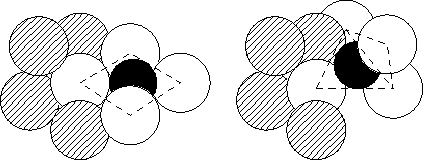
\includegraphics[width=.8\linewidth]{figures/Chapter2/cageeffect}
	\caption{Solvent cage effect in excited state thermal equilibration\,\cite{adamson-1983}.}
	\label{fig:cageeffect}	
\end{wrapfigure}

When light is absorbed by species $A$, a population of $ A^*$ states is produced, and we expect the transition to be a ``vertical" one, that is, electronic rearrangement occurs but no appreciable nuclear motion. Transitions occur in about $10^{-15}$\,s,\footnote{The velocity of an electron making one complete circuit in a Bohr orbit is $\sim 10^{16}$\,\AA/sec. Thus, an electron may move on the order of $10$\,{\AA} in $10^{-15}$\,sec. Since $10$\,{\AA} is the order if size of many commonly encountered groups of atoms (chromophores) responsible for absorption of light, we deduce that the timescales of photon interaction and electron are of the same order of magnitude.\cite{turro-1991}} a time too short for significant displacement of nuclei. The consequence is that $A^*$ molecules are not produced in their equilibrium geometry and should therefore be highly vibrationally excited. This collections of molecules is called Franck-Condon collection or Franck-Condon state ($A^*_{FC}$).\cite{adamson-1983}\par

Assuming that complex $A$ has a square planar geometry, while the equilibrium geometry of $ A^*$ is tetrahedral. A newly formed $A^*$ complex cannot immediately relax to tetrahedral geometry, solvent molecules have to rearrange themselves around (Figure~\ref{fig:cageeffect}); new solvation sphere must be established. As an estimate, it should take roughly about $200$ vibrational periods or about $1$\,ps for a solvent molecule to make diffusional jump from one position to another. The $A^*$ complex is formed in the ground state geometry in a solvent cage that delays its relaxation to the equilibrium geometry. One could expect the collection of molecules $ A^*_{FC}$ to make a succession of configurational adjustments before settling down into an equilibrium Boltzmann distribution of vibrational states. The whole process may take about $10$\,ps. Thermally equilibrated $A^*$ is a thermodynamic state; it represents an ensemble of $A^*$ molecules that is at ambient temperature with respect to vibrations (a solvated molecule really does not have translation or free rotation).\cite{adamson-1983}\par

A representation of molecular electronic state energy levels, with singlet and triplet states in separate columns, is referred to as the Perrin-Jablonski diagram (Figure~~\ref{fig:jablonski-example}). Often, vibrational sublevels are shown schematically as well. Radiative transitions from one level to another are indicated by straight arrows and non-radiative ones by wavy arrows. Most often, the levels correspond to vibrationally relaxed electronic states, \ie to an equilibrium geometry of each individual state. Sometimes, an effort is made to show the state energies at two or more geometries, and as this representation becomes more elaborate, the diagram gradually turns into a drawing of a slice through potential energy surfaces (Figure~\ref{fig:potential-surface}).

\inputfiguresE[1]{Chapter2/Jablonski_cool}{Chapter2/abs-spec}[One possible form of a Perrin-Jablonski diagram, where $I_\pi$ -- ionisation level, $T$ -- triplet and $S$ -- singlet state][The relationship of observed radiative transitions to potential energy curves (schematic)\,\cite{montalti-book-2006}][jablonski-example][potential-surface][.49][.49]


\label{sec:2ch-data}
\inputfigure[1]{Chapter2/RuIandII-emission-77K}[Data for molecules presented on Fig.~\ref{fig:molecules}][RuIandII-emission-77K][pdf]

\begin{equation}
\label{eq:one-level}
\dfrac{dN_1(t)}{dt}=\sigma I(t)-k_1N_1(t)
\end{equation}


Solution of equation~\ref{eq:one-level} is expressed in equation~\ref{eq:solution-one-level}:

\begin{equation}
\label{eq:solution-one-level}
N_1(t)=\dfrac{\sigma \tau_pI_0}{4}\sqrt{\dfrac{\pi}{\ln 2}\exp\left(\dfrac{k_1^2 \tau_p^2}{16\ln2}\right)}\left(1+\erf\left(2\sqrt{\ln 2}\dfrac{t}{\tau_p}-\dfrac{k_1\tau_p}{4\sqrt{\ln2}}\right)\right)\exp(-k_1t)
\end{equation}

To extract deexcitation rate $k_1$ from such function is a complicated mathematical task. Instead of determining $k_1$ as an analytical function, we determined it in an iterative manner, by fitting experimental data as following:

\[
\dfrac{N_{i+1}(t)-N_{i}(t)}{\delta t}=\sigma I(t)-k_1N_i(t),
\]

\noindent so:

\[
N_{i+1}(t)=\left(\sigma I(t)-k_1N_{i}(t)\right)\times \delta t +N_{i}(t),
\] 
\noindent where $\delta t$ is the time step, equalled to $\frac{\text{time-scale}}{N_{points}}$.


\section{Conclusion}
\label{sec:2ch-conslusion}

According to presented data (see Table~\ref{table:Ranges}) we can make conclusions...(see Fig.~\ref{fig:conclusion}).


\inputfigure[1]{Chapter2/PET-Foldamers}[Model for PET in foldamers][conclusion][pdf]



\newpage



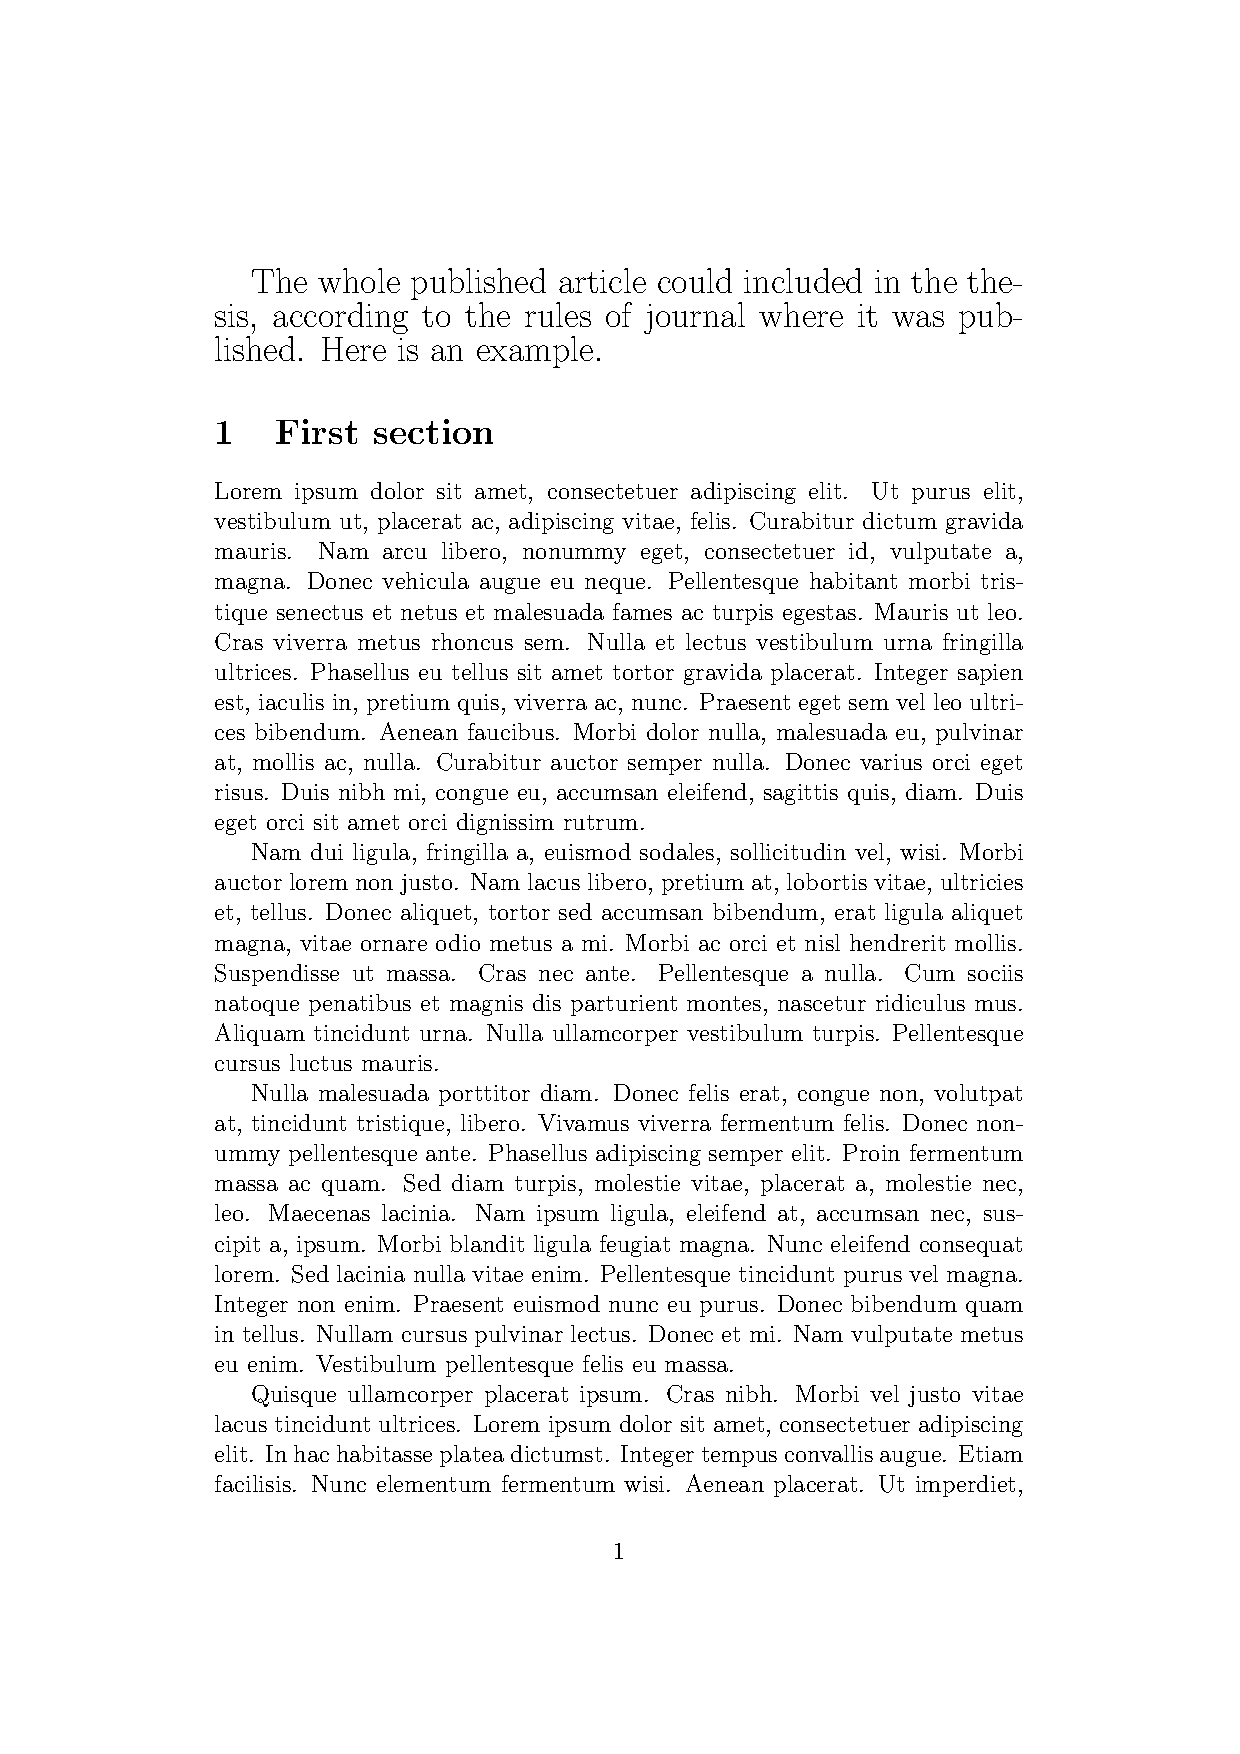
\includepdf[fitpaper=false, pages=-, pagecommand={\thispagestyle{fancy}}, addtotoc={1,section,1,First section, first-sec, 2, section, 1, Second section, sec-sec,2,subsection,2,New subsection,subsec,3,section,1, Third section, third-sec}]{article.pdf}

\stopcontents[chapter]




%APPENDIXES
\appendix
\chapter{Supporting information}
\label{app:Support}
\section{Supporting information}
\label{sec:appSupport-support}
\lipsum[1-2]

\section{Extra}
\label{sec:appSupport-extra}
\lipsum[1-2]

\backmatter
\pagestyle{plain}

\addcontentsline{toc}{chapter}{\bibname}
\begingroup
\setstretch{1}
\setlength\bibitemsep{0pt}
\renewcommand*{\bibfont}{\small}
\sloppy %Line breaking
\printbibliography
\endgroup


%INDEXES
\printindex[cite]
%\printindex[pms]


%Glossary
\glsaddall
\renewcommand*{\glsgroupskip}{}
\printglossary[title=Abbreviations, toctitle=Abbreviations, type=\acronymtype, style=list]



\end{document}